\section{Introduction}

Computer malwares are always big threats to individual and organizational users. For example, a worn or virus can cause system crash leading to data loss; a trojan or a malicious URL can steal user's sensitive  information leading to economic loss. In 20xx, the loss cause by xxx is about xxxx. Effort to combating malwares have never stopped, and industrial companies and research communities have made various achievements. ~\ref{xxx}\wenfei{check reviewers' publications and put them here.}

Malwares are still increasing exponentially now, but our effort does scale with the rapidly worsening situation. For example, the volume of mobile malwares tripled in 2015, while the revenue spent on malware research increased only by about 10\% each year. 
To focus the effort in anti-malware research and engineering, systematic measurement studies are necessary to guide practices. For example, if a anti-malware company can know the malwares that will be prevailing in the current or next time period, they would be able to focus on these malwares.
However, there are few of such studies to reveal malware characteristics and the characterization methodology now. 

In this paper, we make an empirical study of a malware dataset from VirusTotal. VisualTotal is a free online service using antivirus engines from security companies to identify submitted suspicious malwares.
We first made use of VirusTotal public API to collect a malware dataset in November, 2015. Our dataset collection focuses on Windows executables and libraries and their analysis result by Microsoft antivirus engine to guarantee accuracy. 

We perform an analysis on the characteristics of the VirusTotal dataset. In addition to general characteristics such as malware family (i.e. category, defined in Section xx) distribution and the generation rate of new malware families, we specifically look into the temporal characteristics of the malware dataset, and find that there is obvious time locality. That is, current malware families are more likely to appear in the next time period.

We then made a study of hot malware family mining algorithms. We compare the performance of frequent item mining algorithm with exhaustive counting algorithm. Our results show that, we acceptable penalty the frequent item mining algorithm gives satisfactory predictive result in terms of memory space. 

\wenfei{edit until here}

In this paper, we view data on VirusTotal as a stream, based on each file’s submission time, and design two stream mining applications: 
\textit{hot malware family mining} and \textit{malware prediction}. 
There are possibly infinite malware families. 
Hot malware family mining can precisely identify malware families, 
which occupy more than a given percentage of total malwares, by using a constant number of counters.
Malwares does not appear uniformly across different malware families or across time, 
and they appear in bursts. 
We built a cache-based algorithm to predict malwares in which families would appear in the near future. 

\begin{figure}[t!]
\begin{center}
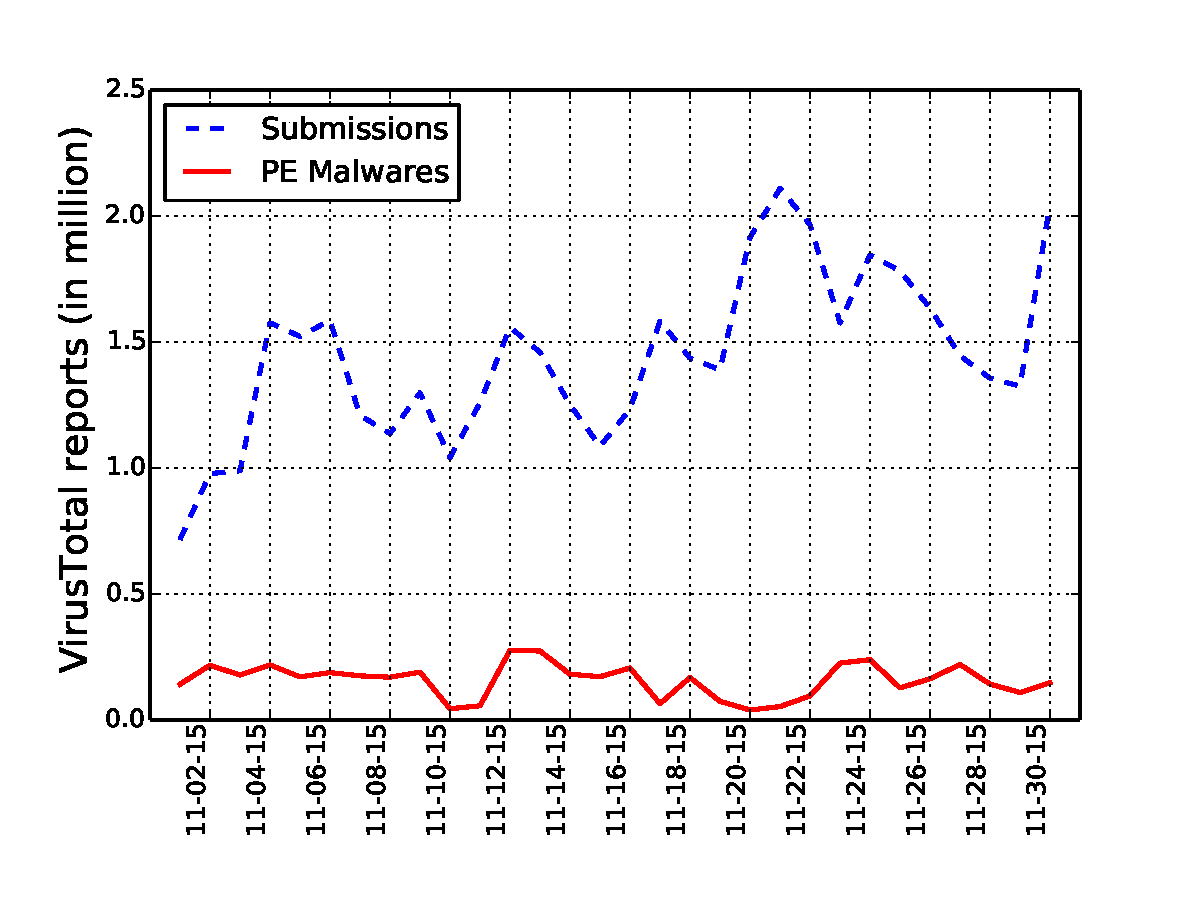
\includegraphics[width=3.0in]{figure/nov}
\caption{The number of files submitted to VirusTotal last November. }
\label{fig:subnum}
\end{center}
\end{figure}

In summary, we made the following contributions in this paper:

\begin{itemize}

\item We collect data submitted to VirusTotal last November, 
and briefly analyze these data to understand the characteristics of VirusTotal repository (Section~\ref{sec:meth}). 
\item We build two stream mining applications, one could identify hot malware family in a constant number of counters (Section~\ref{sec:hot}), 
and the other could predict malwares in the near future (Section~\ref{sec:predict}). 
Experimental results show that we can cover all hot malware family with a very few false positives, and we can predict future malwares with a high precision.
\item We discuss the future research opportunities through mining data on VirusTotal (Section~\ref{sec:oppo}), 
and demonstrate the feasibility by using our experience of building stream mining applications. 

\end{itemize}



